\chapter{Analisis dan Perancangan}

\section{Analisis Malware WannaCry}

Pada bagian ini, peneliti memfokuskan analisa malware WannaCry pada analisa lalu lintas paket yang dilakukan oleh host terinfeksi. Analisis malware WannaCry dilakukan dengan melakukan \textit{sniffing} dengan menggunakan 3 host dengan jaringan terisolasi seperti pada gambar \ref{fig:analisis_malware_net}. Ketiga host tersebut memiliki arsitektur yang sama yakni x86\_64 sehingga tidak ada alignment (seperti little endian dan big endian) berbeda.

\begin{figure}[H]
	\centering
	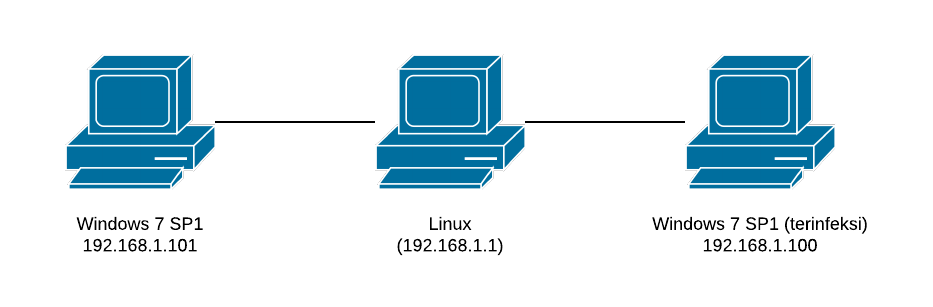
\includegraphics[width=400px]{resources/analisis_malware_net.png}
	\caption{Susunan jaringan untuk analisis malware WannaCry}
	\label{fig:analisis_malware_net}
\end{figure}

Host linux (192.168.1.1) menjadi host dengan dua interface yang dijadikan \textit{bridge}. Sehingga host Windows 7 terinfeksi (192.168.1.100) dapat berkomunikasi dengan host Windows 7 SP1 (192.168.1.101) hanya melalui 192.168.1.1. Kemudian pada host linux dilakukan sniffing dengan menggunakan tcpdump. dengan command sebagai berikut:

\begin{verbatim}
$ tcpdump -s0 -i br0 -vv -w output.wannacry-1.pcap
\end{verbatim}

\section{Karakteristik Malware WannaCry}

Dari pengelompokan malware menjadi worm, virus dan trojan horse menurut (\cite{idika2007survey}) maka WannaCry digolongkan sebagai worm. Sesuai dengan karakteristik yang disebutkan WannaCry memiliki kapabilitas menginfeksi melalui network. WannaCry memiliki dua buah bagian utama: ransomware, dan worm penginfeksi, yang melakukan penyebaran melalui protokol SMB. Jika sebuah host hanya menjalankan bagian ransomware saja, maka tidak akan ada penyebaran yang dilakukan, seperti ditunjukan pada Gambar \ref{fig:no_infect_action}. Sedangkan jika host menjalankan bagian dropper, dropper tersebut akan menjalankan worm penginfeksi dan sekaligus menjalankan ransomware. Pada Gambar \ref{fig:infect_action} terlihat host 192.168.1.100  mencoba melakukan koneksi ke port \verb|445/tcp| setiap host yang berada pada subnet yang sama.

\begin{figure}[H]
	\centering
	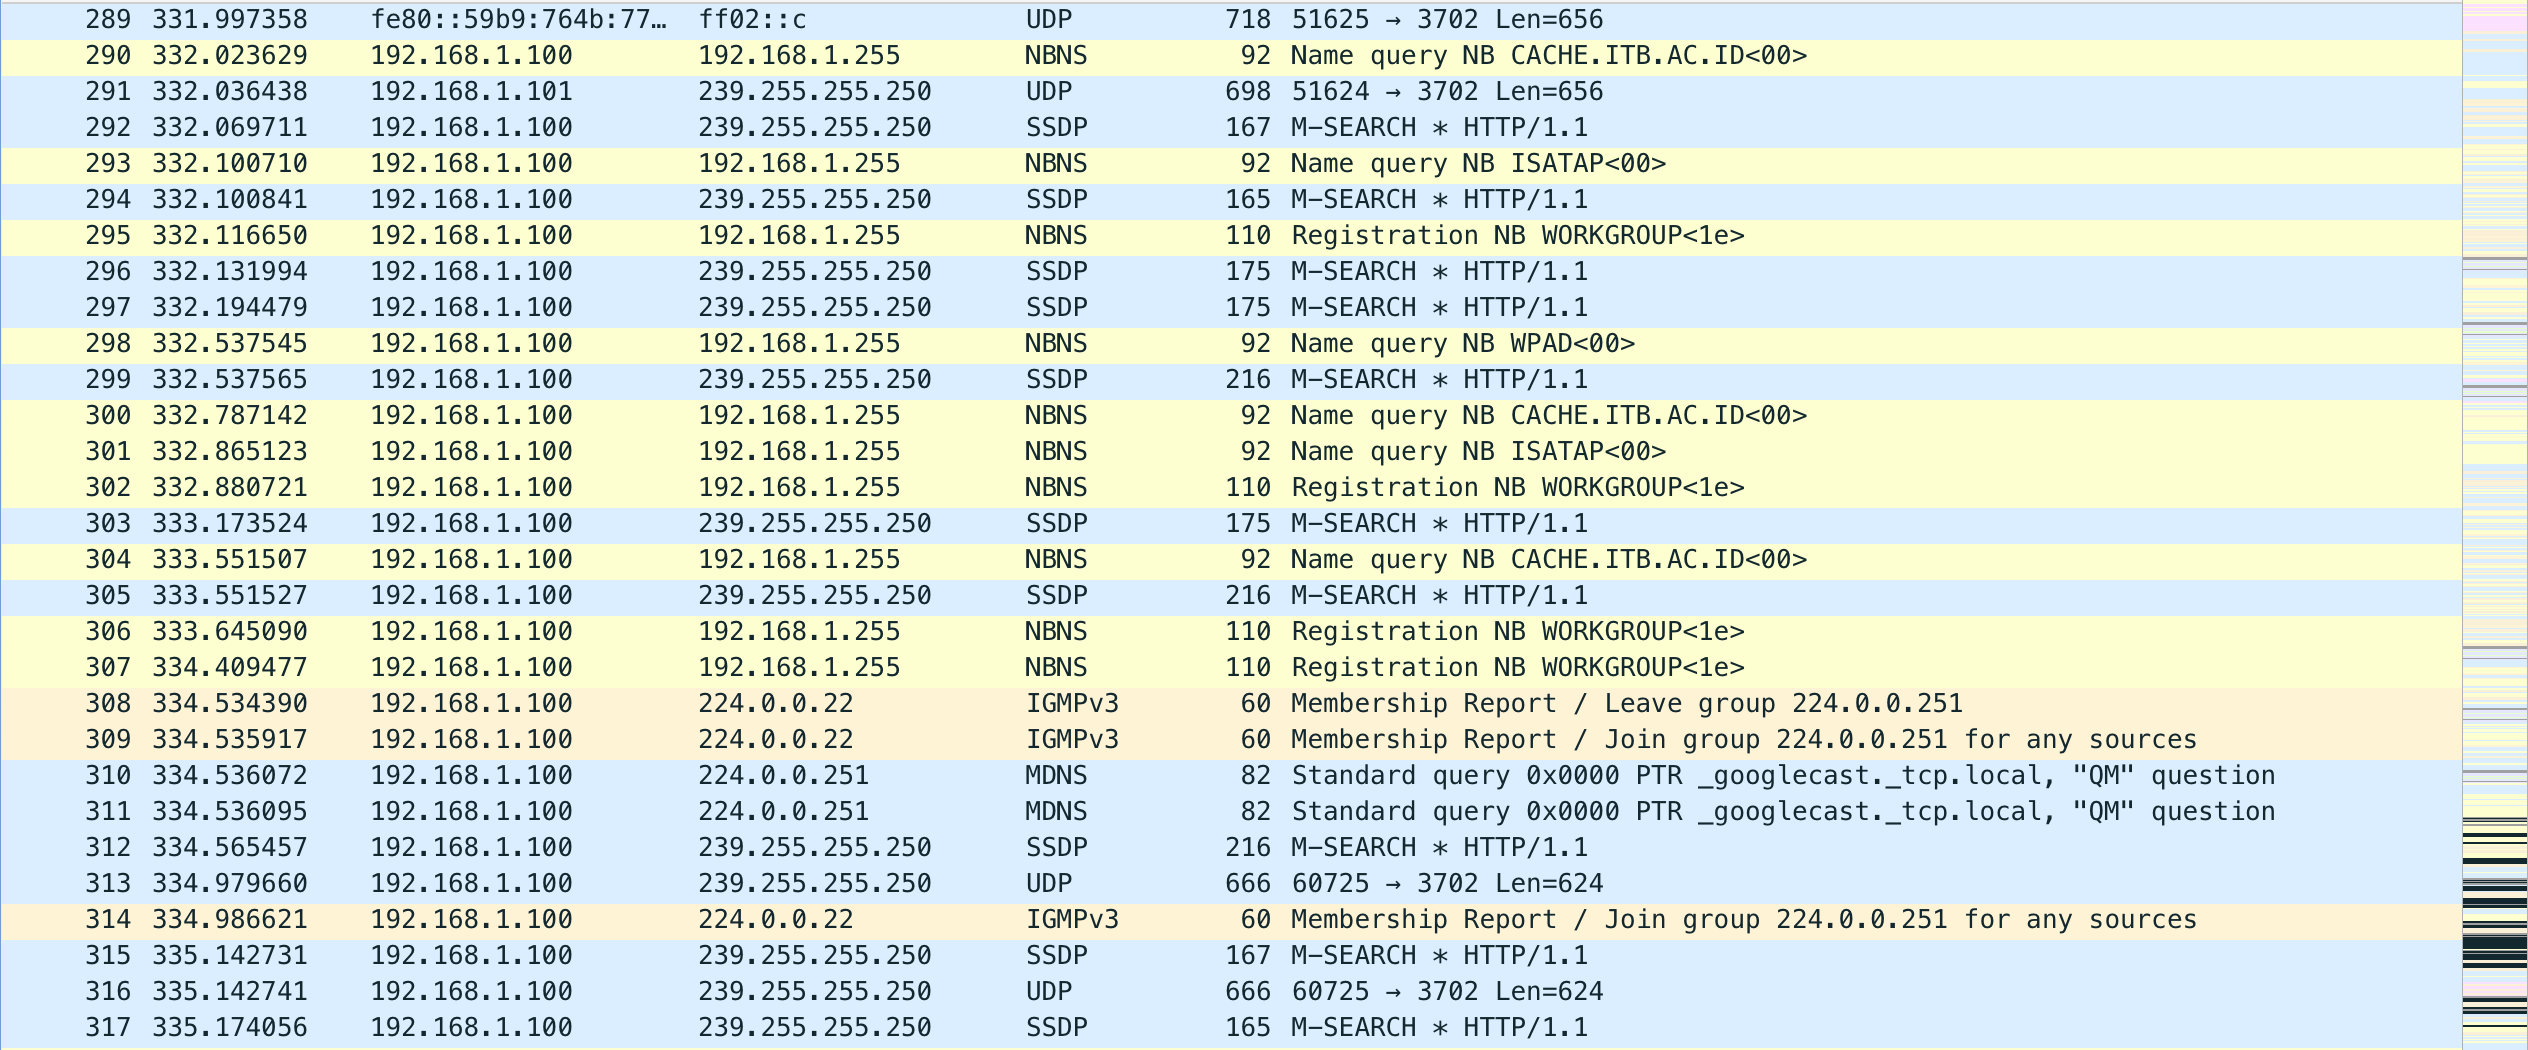
\includegraphics[width=\textwidth]{resources/no_infect_action.png}
	\caption{Paket pada host terinfeksi ransomware tanpa worm penginfeksi}
	\label{fig:no_infect_action}
\end{figure}

\begin{figure}[H]
	\centering
	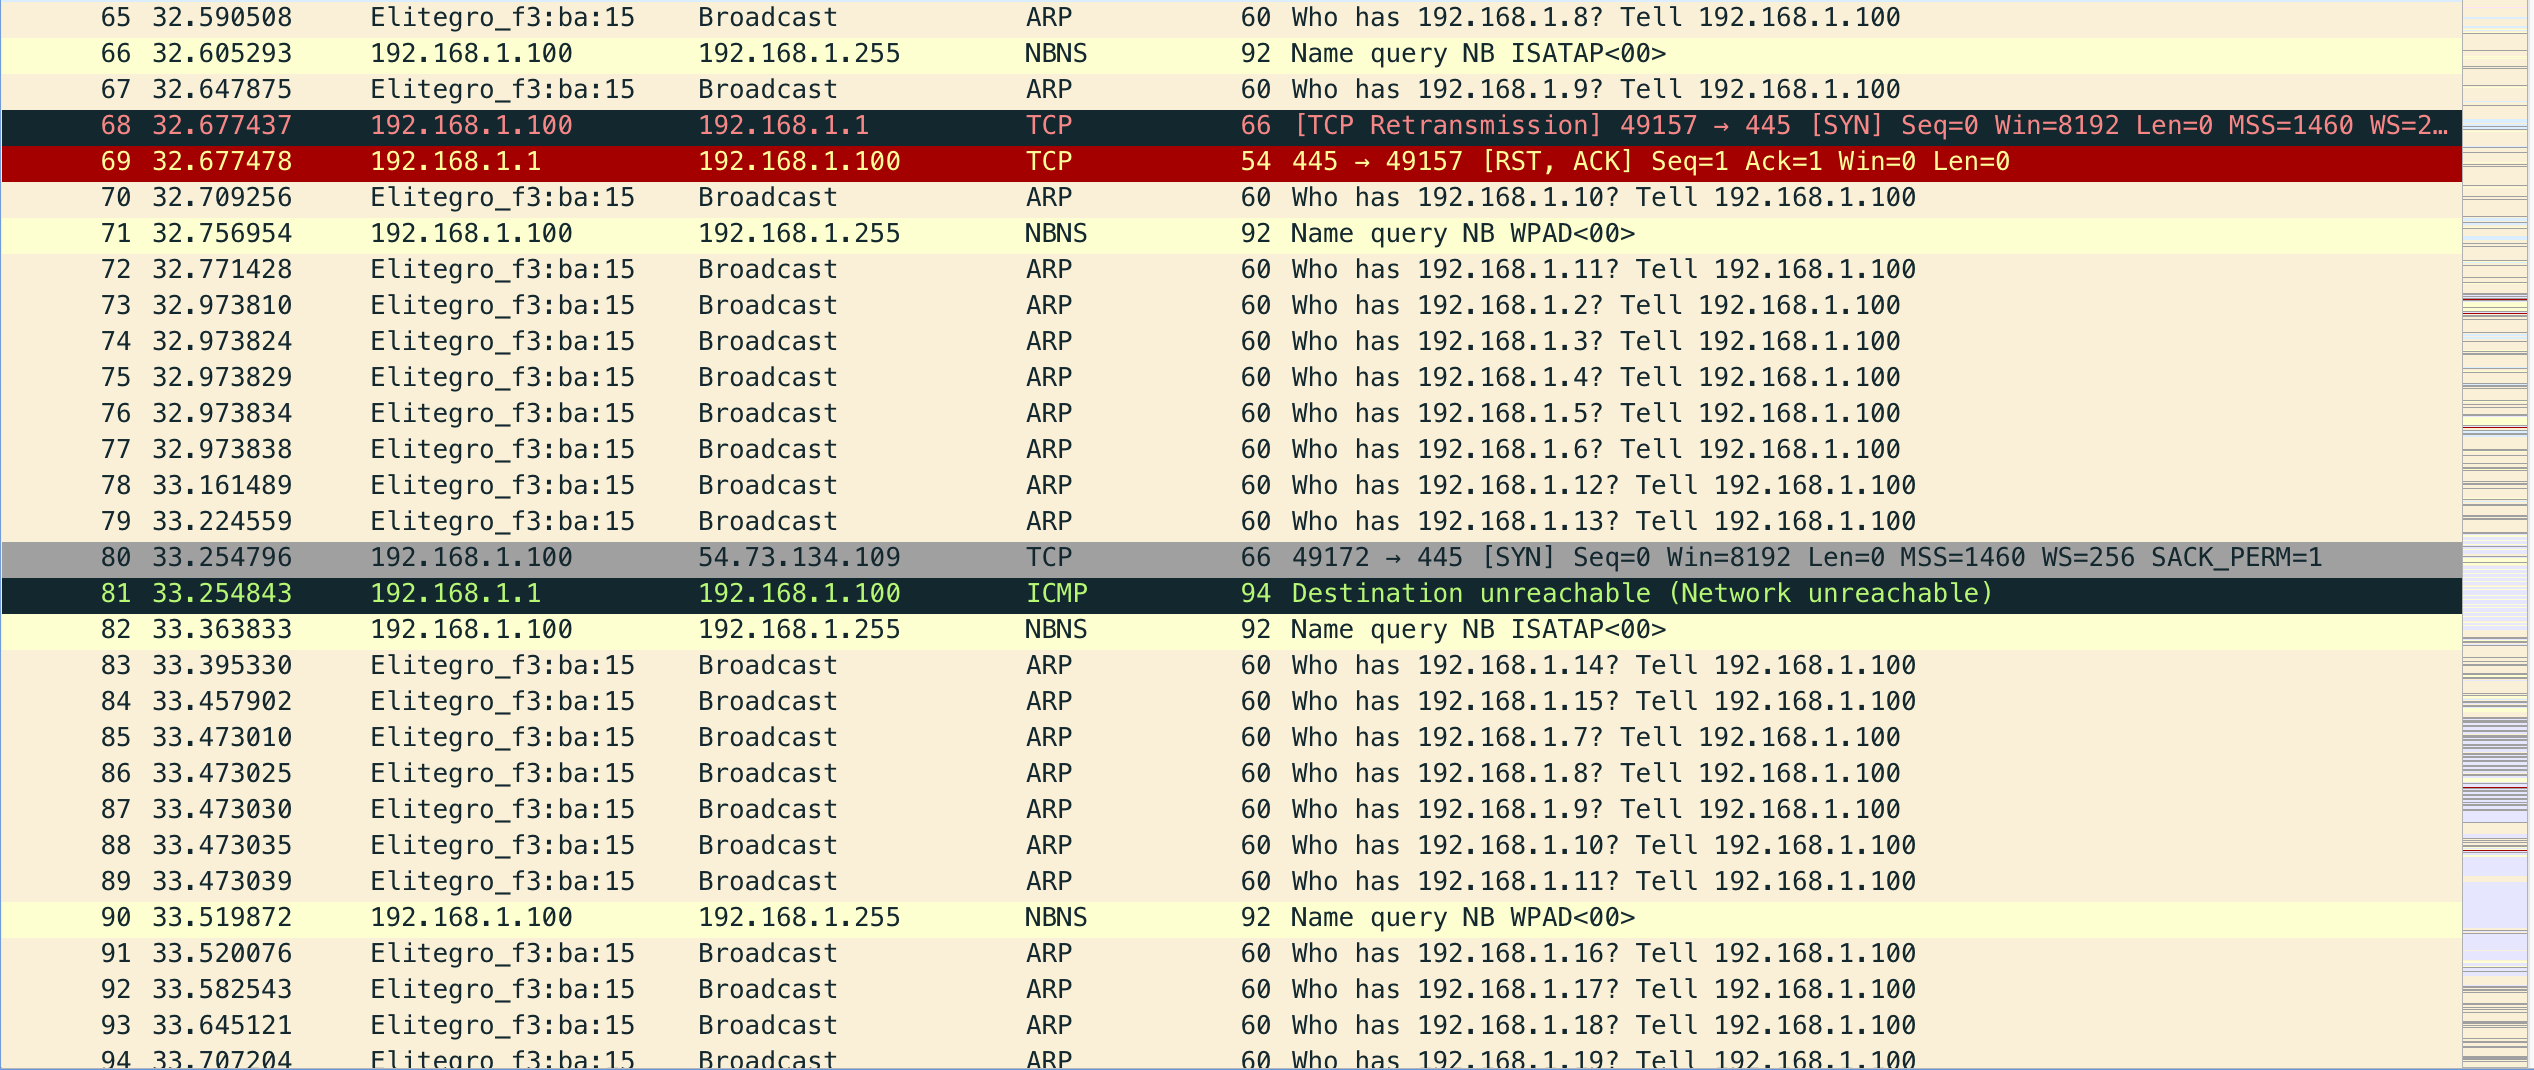
\includegraphics[width=\textwidth]{resources/infect_action.png}
	\caption{Paket pada host terinfeksi ransomware dengan dropper}
	\label{fig:infect_action}
\end{figure}

Ransomware merupakan kategori malicious software yang ketika dijalankan akan menonaktifkan fungsi tertentu dari komputer dengan sebuah cara. Kemudian ransomware akan menampilkan pesan untuk meminta pembayaran untuk mengembalikan fungsi yang dinonatifkan. Sehingga malware seakan-akan melakukan penyandraan terhadap komputer. (\cite{o2012ransomware}).

Dari riset yang telah dilakukan oleh \cite{islam2018smb}, WannaCry melakukan exploit terhadap vulnerability yang menurut EternalBlue dan DoublePulsar yang ada pada implementasi SMB1.

\subsection{Vulnerability EternalBlue}
EternalBlue merupakan vulnerability yang diakibatkan oleh 3 buah bug (\cite{islam2018smb}) dan (\cite{grossman2017check}) yakni:
\begin{enumerate}
	\item Wrong casting bug
	\item Wrong parsing function bug
	\item Non-paged pool allocation bug
\end{enumerate}

Pada host 192.168.1.100 paket yang dikirimkan malware untuk mengeksploitasi vulnerability seperti yang disebutkan (\cite{islam2018smb}) terlihat pada Gambar \ref{fig:trans_nop}.

\begin{figure}[H]
	\centering
	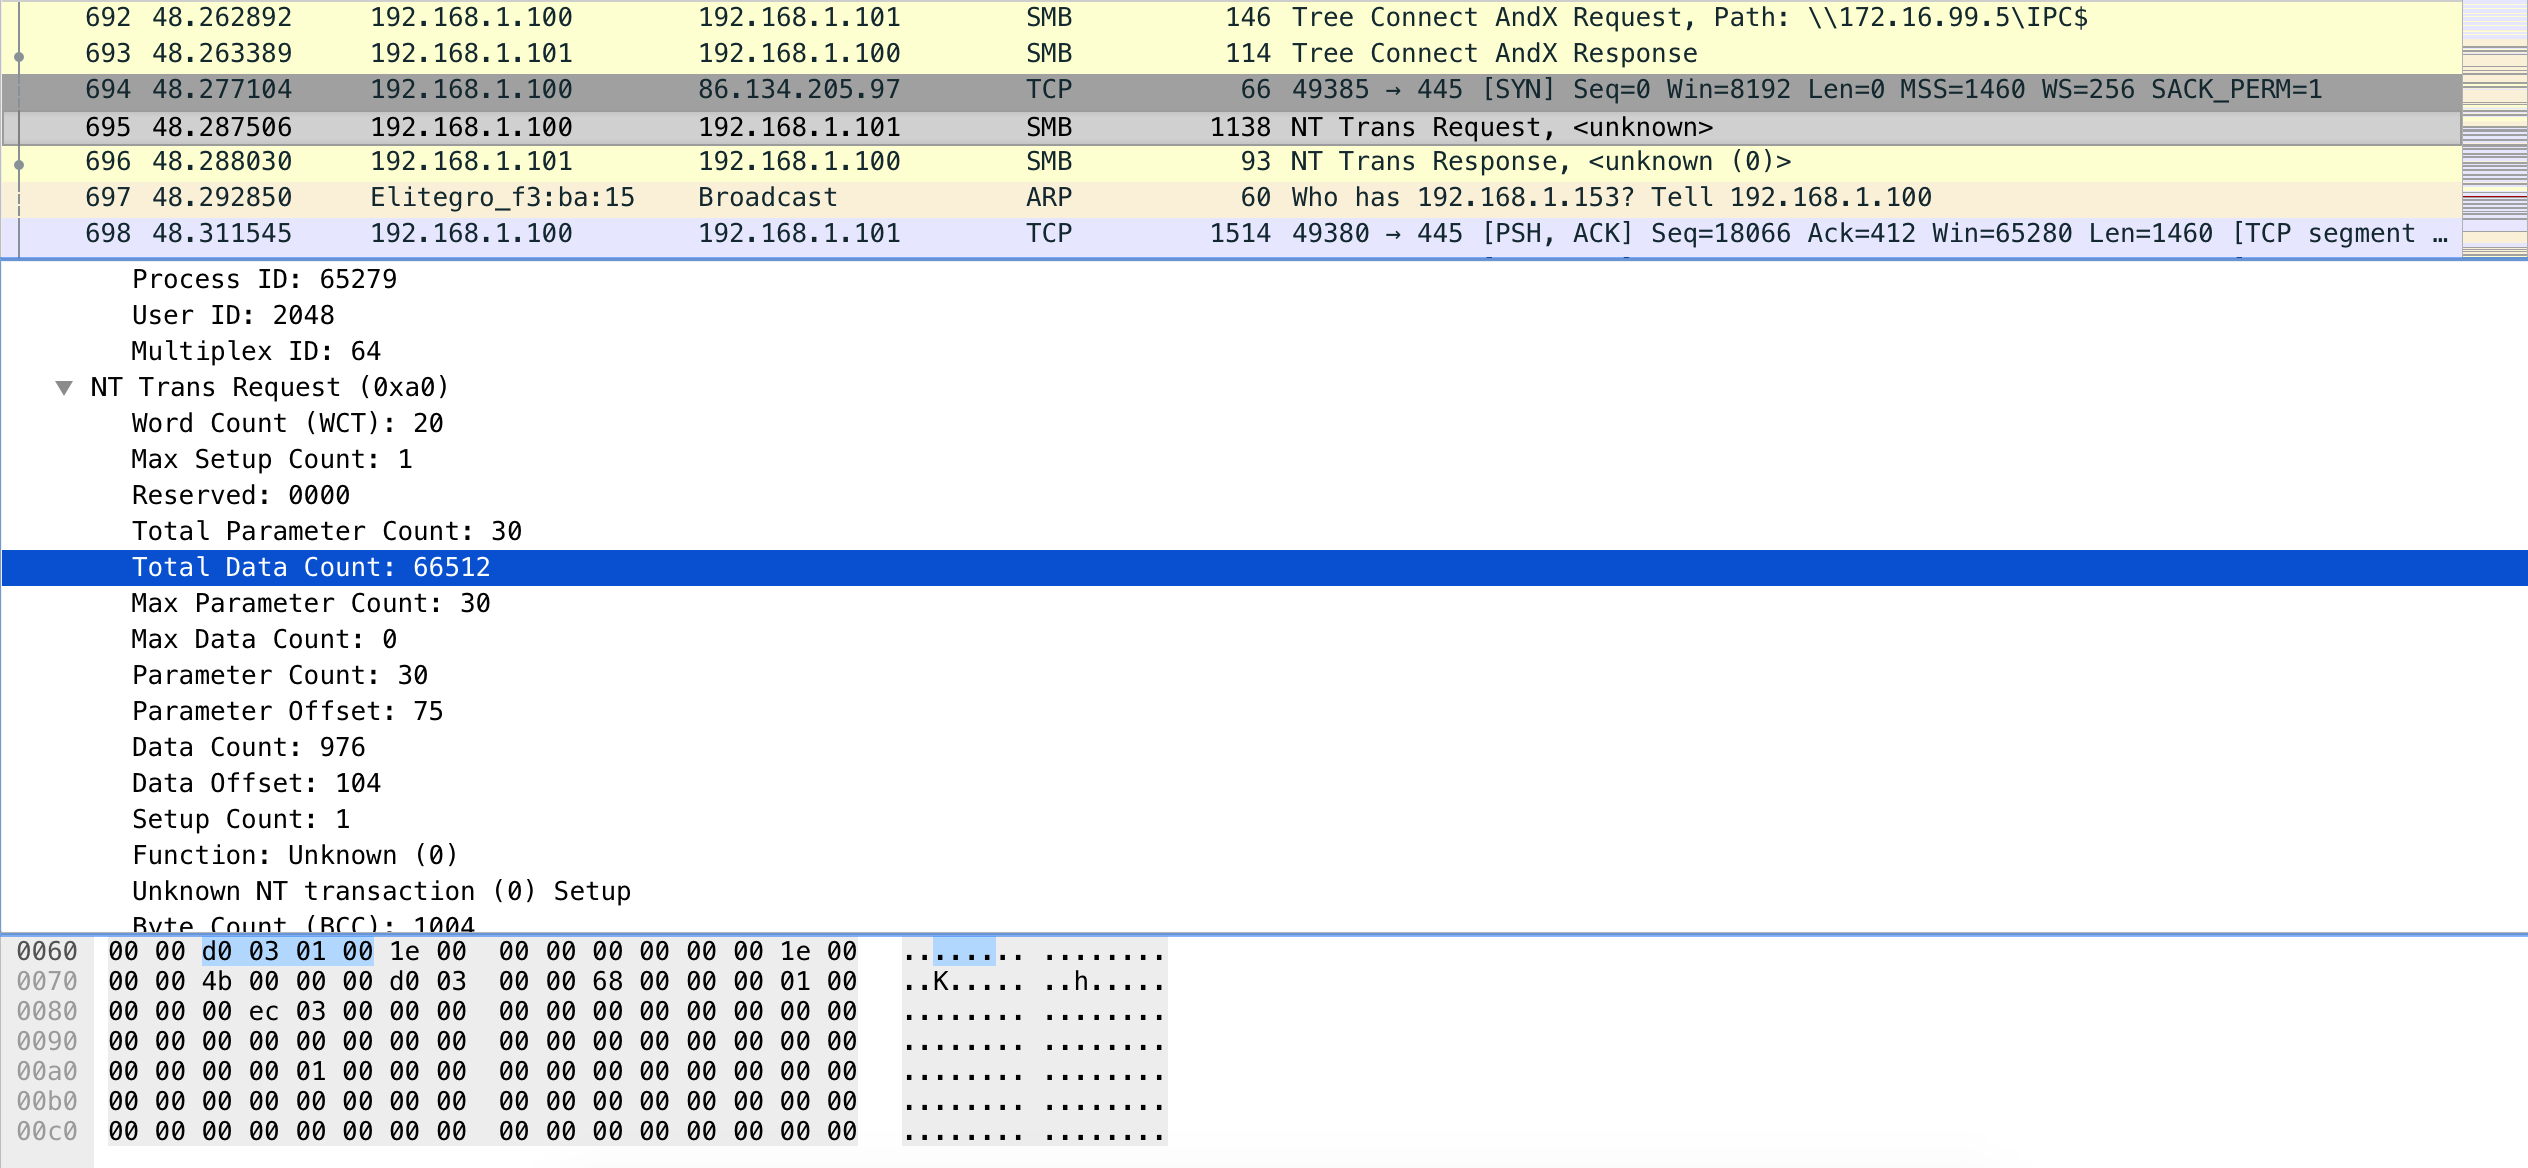
\includegraphics[width=\textwidth]{resources/trans_nop.png}
	\caption{Paket pada host terinfeksi ransomware dengan dropper}
	\label{fig:trans_nop}
\end{figure}


\subsection{Vulnerability DoublePulsar}

\section{Analisis Payload SMB oleh WannaCry}

Pada malware wannacry

\section{Deteksi Protokol oleh nDPI}

\section{Deteksi signature dengan string matching}


\section{Penangkalan paket \textit{malicious} dengan firewall}


\section{Penentuan rule iptables untuk melakukan \textit{block} pada \textit{payload} WannaCry}


